%!TEX root = 00_main.tex

\section{Experiments}

\commentA{the distribution figures would be nice here, e.g. to make the point that we can synthesise arbitrary distributions and to beef up the gaze estimation experiments}
\begin{figure*}
    \centering
    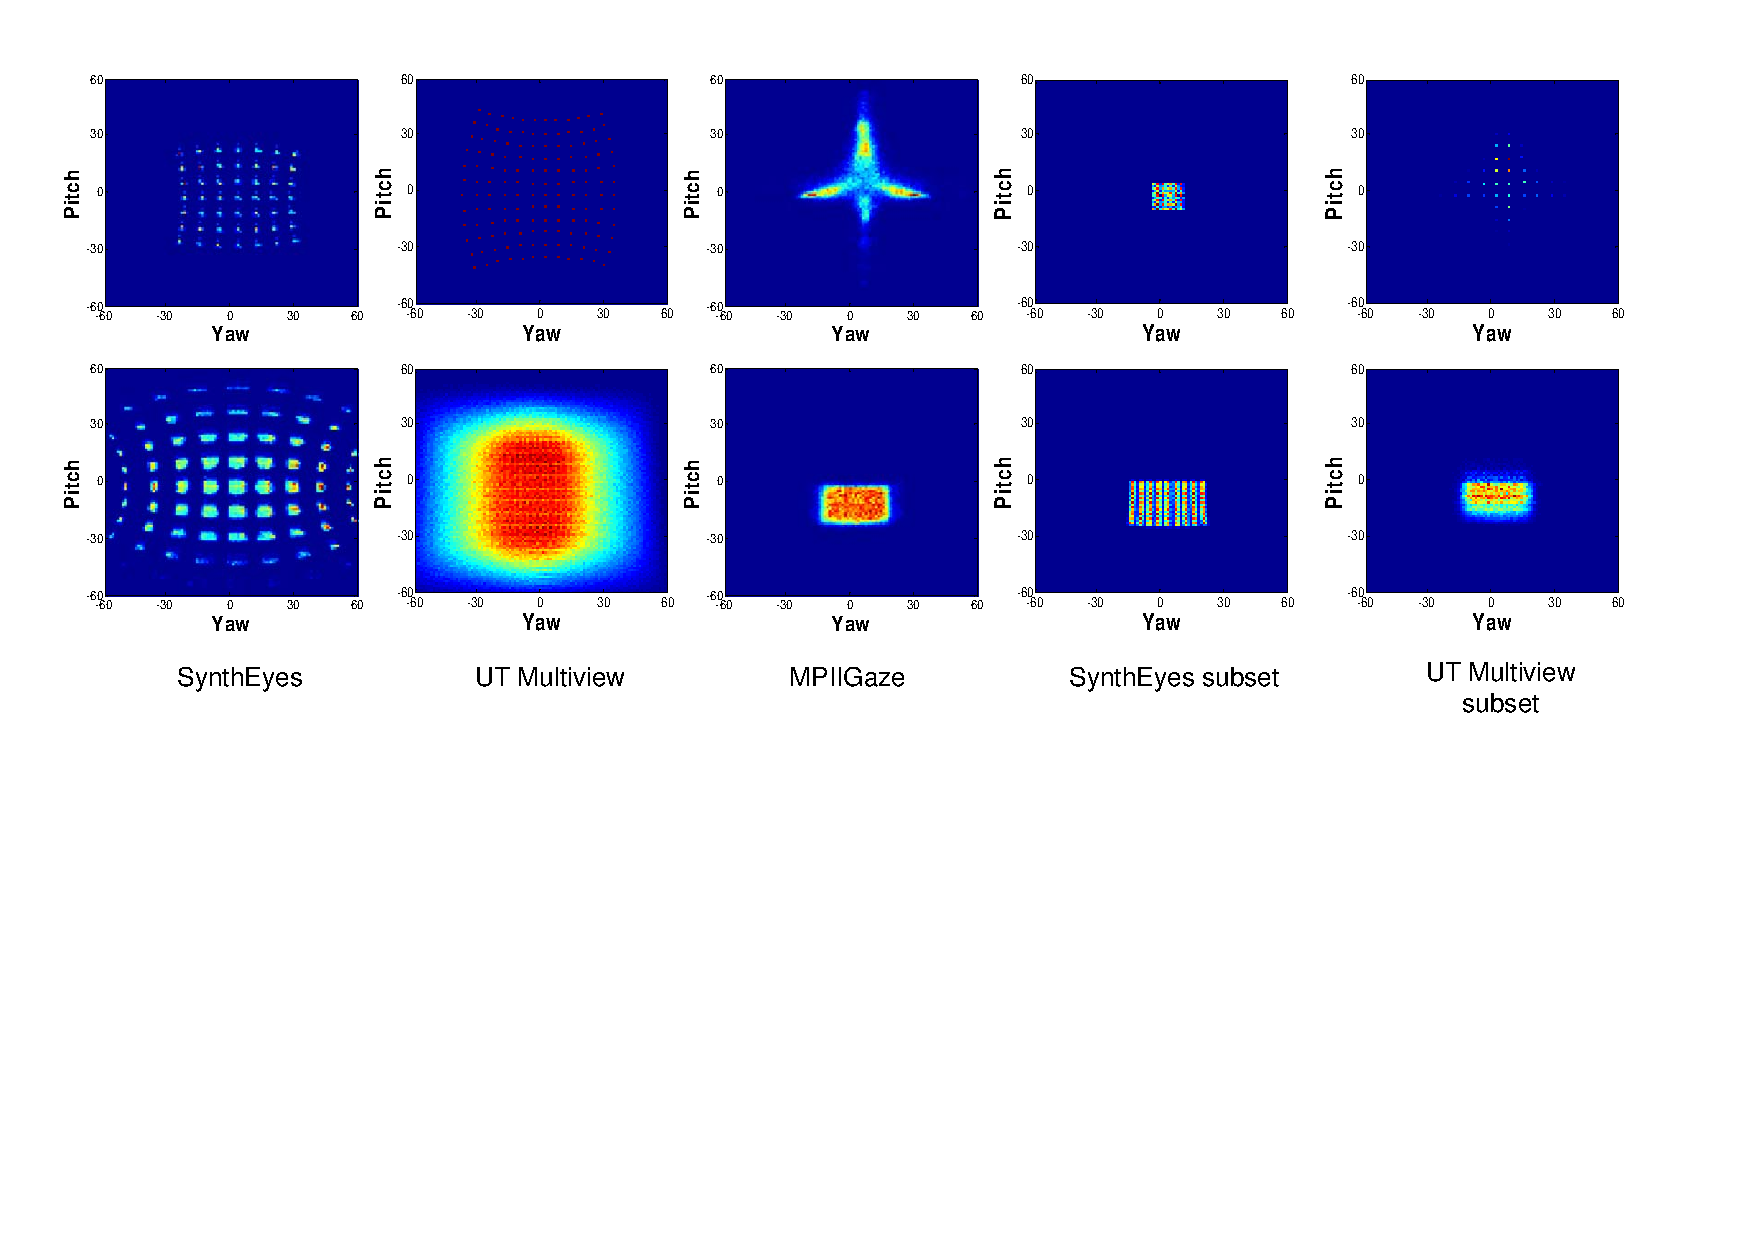
\includegraphics[width=\textwidth]{head_gaze_distribution.pdf}
    \caption{The head pose (first row) and gaze direction (second row) distribution of different datasets.}
    \label{fig:gazeResult}
\end{figure*}


% \begin{figure}
    \centering
    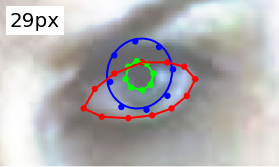
\includegraphics[width=0.244\columnwidth]{figs/wild_ldmks_examples/idx_550.png}\hfill
    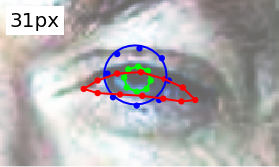
\includegraphics[width=0.244\columnwidth]{figs/wild_ldmks_examples/idx_560.png}\hfill
    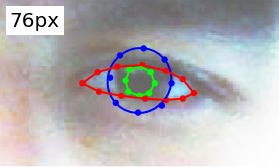
\includegraphics[width=0.244\columnwidth]{figs/wild_ldmks_examples/idx_799.png}\hfill
    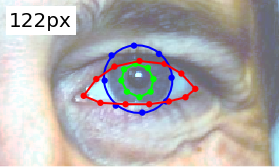
\includegraphics[width=0.244\columnwidth]{figs/wild_ldmks_examples/idx_721.png}
    \par \vspace{0.1em}
    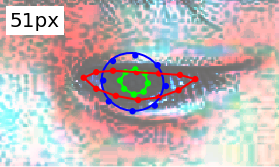
\includegraphics[width=0.244\columnwidth]{figs/wild_ldmks_examples/idx_1013.png}\hfill
    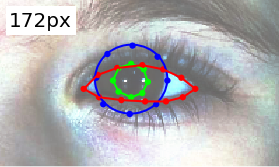
\includegraphics[width=0.244\columnwidth]{figs/wild_ldmks_examples/idx_1002.png}\hfill
    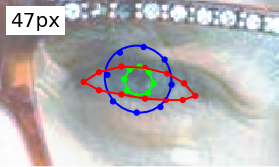
\includegraphics[width=0.244\columnwidth]{figs/wild_ldmks_examples/idx_765.png}\hfill
    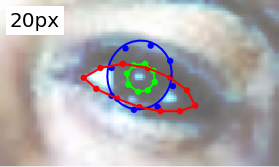
\includegraphics[width=0.244\columnwidth]{figs/wild_ldmks_examples/idx_508.png}
    \par \vspace{0.1em}
    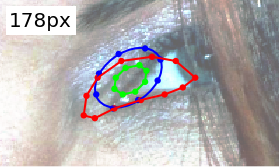
\includegraphics[width=0.244\columnwidth]{figs/wild_ldmks_examples/idx_934.png}\hfill
    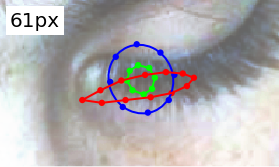
\includegraphics[width=0.244\columnwidth]{figs/wild_ldmks_examples/idx_875.png}\hfill
    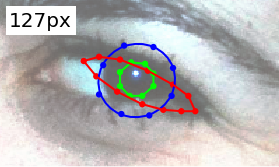
\includegraphics[width=0.244\columnwidth]{figs/wild_ldmks_examples/idx_913.png}\hfill
    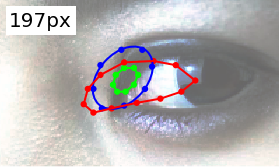
\includegraphics[width=0.244\columnwidth]{figs/wild_ldmks_examples/idx_953.png}
    %
    \caption{The top two rows illustrate successful eye-shape registration on 300-W. The bottom row illustrates failure cases, including un-modelled occlusions and eyelid poses.}
    \label{fig:example_fits_wild}
\end{figure}

We evaluated the usefulness of our synthetic data generation method on two sample problems, eye-shape registration and appearance-based gaze estimation.

\commentA{briefly say something about significance/importance of both problems, more in corresponding subsections}

\subsection{Eyelid Registration In the Wild}

\begin{figure}
    \centering
    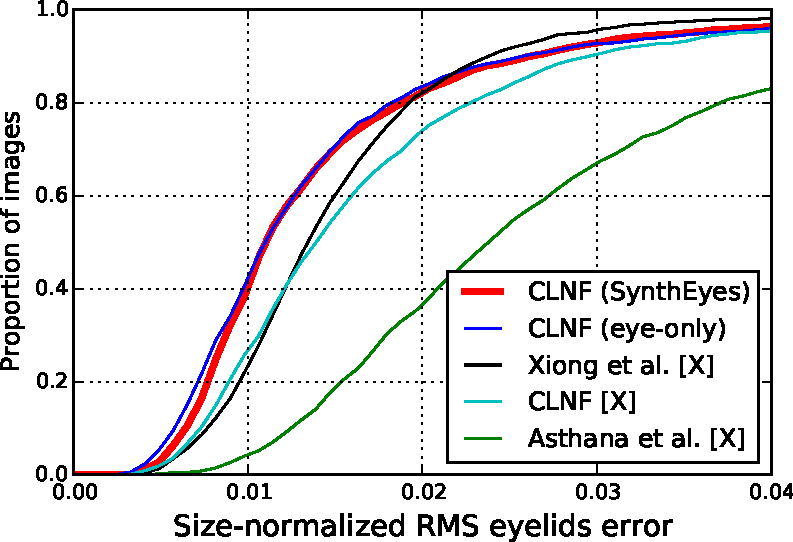
\includegraphics[width=\columnwidth]{figs/CLNF_300W_experiment.pdf}
    \caption{Results of 300-W experiment}
    \label{fig:clnf_results_wild}
\end{figure}

\begin{figure}
    \centering
    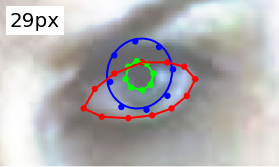
\includegraphics[width=0.244\columnwidth]{figs/wild_ldmks_examples/idx_550.png}\hfill
    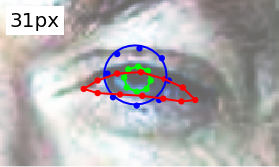
\includegraphics[width=0.244\columnwidth]{figs/wild_ldmks_examples/idx_560.png}\hfill
    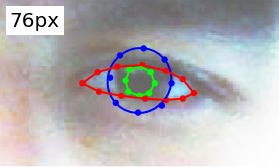
\includegraphics[width=0.244\columnwidth]{figs/wild_ldmks_examples/idx_799.png}\hfill
    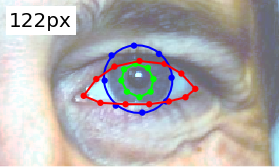
\includegraphics[width=0.244\columnwidth]{figs/wild_ldmks_examples/idx_721.png}
    \par \vspace{0.1em}
    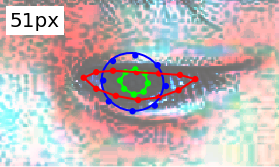
\includegraphics[width=0.244\columnwidth]{figs/wild_ldmks_examples/idx_1013.png}\hfill
    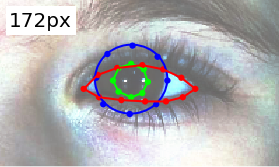
\includegraphics[width=0.244\columnwidth]{figs/wild_ldmks_examples/idx_1002.png}\hfill
    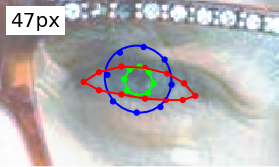
\includegraphics[width=0.244\columnwidth]{figs/wild_ldmks_examples/idx_765.png}\hfill
    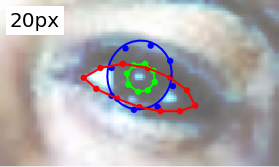
\includegraphics[width=0.244\columnwidth]{figs/wild_ldmks_examples/idx_508.png}
    \par \vspace{0.1em}
    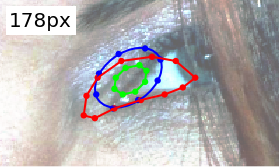
\includegraphics[width=0.244\columnwidth]{figs/wild_ldmks_examples/idx_934.png}\hfill
    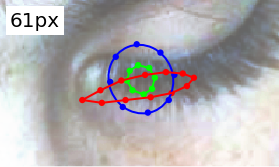
\includegraphics[width=0.244\columnwidth]{figs/wild_ldmks_examples/idx_875.png}\hfill
    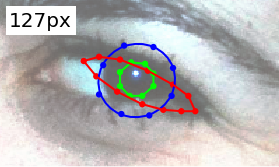
\includegraphics[width=0.244\columnwidth]{figs/wild_ldmks_examples/idx_913.png}\hfill
    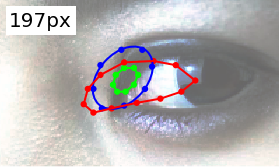
\includegraphics[width=0.244\columnwidth]{figs/wild_ldmks_examples/idx_953.png}
    %
    \caption{The top two rows illustrate successful eye-shape registration on 300-W. The bottom row illustrates failure cases, including un-modelled occlusions and eyelid poses.}
    \label{fig:example_fits_wild}
\end{figure}

% Erroll to Tadas: need to make sure these facts are straight...
We performed an experiment to see how our our system generalises on unseen and unconstrained images from the 300 Faces In-the-Wild (300-W) \cite{sagonas2013300} datasets.
We used a generic \dataset dataset for training with 11,382 images rendered with $40^{\circ}$ head pose variation and $90^{\circ}$ gaze variation.
We compared our approach with the following: \todo{briefly list other systems}
The 1026 test images feature 6 eye-region landmarks from the Multi-PIE \cite{gross2010multi} mark-up corresponding to the eyelid boundary. Errors were recorded as the RMS point-to-boundary distance from tracked eyelid landmarks to ground truth eyelid boundary, and were normalized by inter-ocular distance.
To initialize model fitting we first used the face-CLNF \cite{baltrusaitis2013constrained}, which we also use as a baseline.

As shown in \autoref{fig:clnf_results_wild}, the results show the eye-CLNF outperforming all comparison systems in eye-lid localization. \todo{more}. Note that our system trained on only ten participants in four lighting conditions results in comparable performance to a system trained on unconstrained in-the-wild images -- this suggests high-quality labels are important.

Our data synthesis system also allows us to examine what steps of the synthesis approach are important for generating good training data. We trained two further eye-CLNFs on different versions of \dataset, one without eyelid motion and one with only one fixed lighting condition. As can be seen in \autoref{fig:clnf_results_wild}, these perform worse as they are missing important degrees of variability.

\subsection{Eye-Shape Registration for Laptops}

\commentA{``for laptops'' sounds very specific. Does this generalise, do we need this strong constraint?}

\begin{figure}
    \centering
    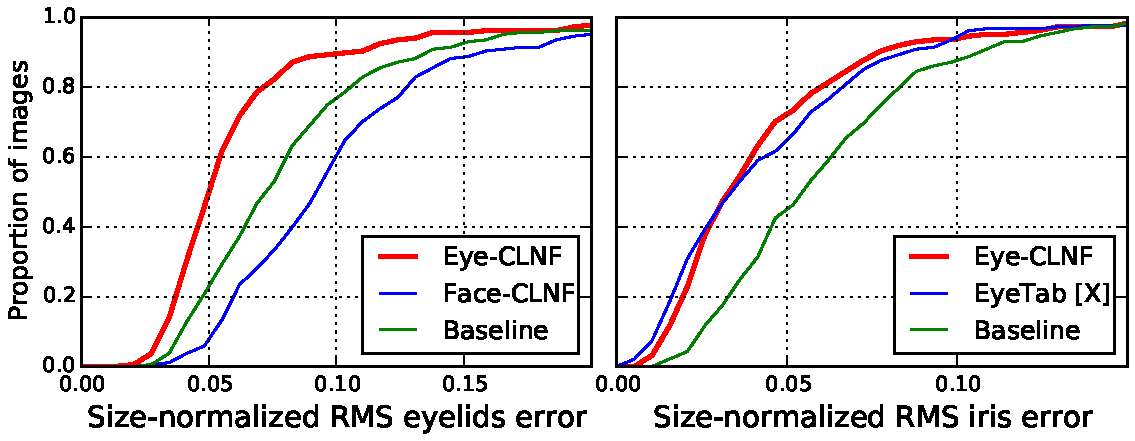
\includegraphics[width=\columnwidth]{CLNF_MPII_experiment}
    \caption{Results of annotated MPII experiment}
    \label{fig:clnf_results_MPII}
\end{figure}

\begin{figure}
    \centering
    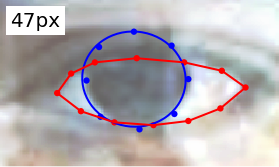
\includegraphics[width=0.244\columnwidth]{figs/ldmks_examples/idx_0.png}\hfill
    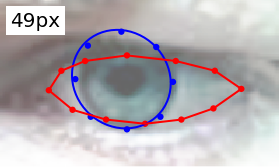
\includegraphics[width=0.244\columnwidth]{figs/ldmks_examples/idx_55.png}\hfill
    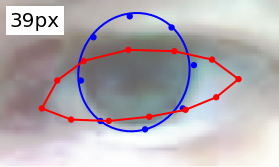
\includegraphics[width=0.244\columnwidth]{figs/ldmks_examples/idx_160.png}\hfill
    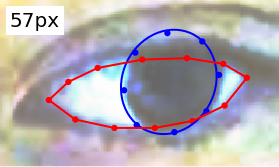
\includegraphics[width=0.244\columnwidth]{figs/ldmks_examples/idx_12.png}
    \par \vspace{0.1em}
    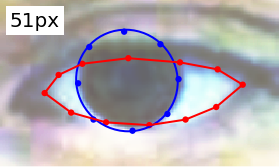
\includegraphics[width=0.244\columnwidth]{figs/ldmks_examples/idx_35.png}\hfill
    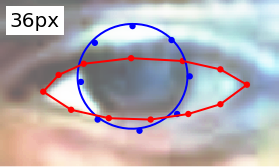
\includegraphics[width=0.244\columnwidth]{figs/ldmks_examples/idx_145.png}\hfill
    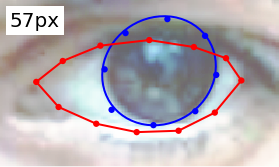
\includegraphics[width=0.244\columnwidth]{figs/ldmks_examples/idx_171.png}\hfill
    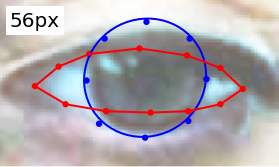
\includegraphics[width=0.244\columnwidth]{figs/ldmks_examples/idx_113.png}
    \par \vspace{0.1em}
    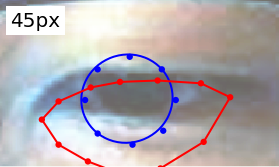
\includegraphics[width=0.244\columnwidth]{figs/ldmks_examples/idx_179.png}\hfill
    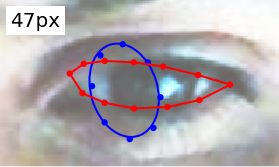
\includegraphics[width=0.244\columnwidth]{figs/ldmks_examples/idx_42.png}\hfill
    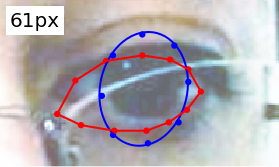
\includegraphics[width=0.244\columnwidth]{figs/ldmks_examples/idx_63.png}\hfill
    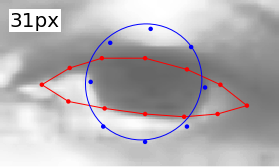
\includegraphics[width=0.244\columnwidth]{figs/ldmks_examples/idx_96.png}
    %
    \caption{The top two rows illustrate successful eye-shape registration on MPIIGaze. The bottom row illustrates failure cases.}
    \label{fig:clnf_examples}
\end{figure}

While the 300-W images represent challenging conditions for eyelid registration, they are not representative of typical webcam-style images and do not feature iris labels.
We therefore annotated sub-pixel eyelid and iris boundaries onto a subset of MPIIGaze ($n\!=\!188$), a recent large-scale dataset of face images and corresponding on-screen gaze locations collected during everyday laptop use over several months~\cite{zhang15_cvpr}.
Pupil accuracy was not evaluated as it was impossible to discern in in most images.
We compared our eye-CLNF with EyeTab \cite{wood2014eyetab}, a state-of-the-art shape-based approach that robustly fits ellipses to the limbus using image-aware RANSAC \cite{swirski2012robust}.
We used the author's implementation, with their suggested modifications: improved eyelid localization with a CLNF facial landmark detector \cite{baltrusaitis2013constrained}.
As a baseline, we used the mean position of all eye-landmarks following model initialization.
Eyelid errors were calculated as RMS distances from eyelid landmarks to the ground truth eyelid boudnary.
Iris errors were calculated by first least-squares fitting an ellipse to the tracked iris landmarks, discretizing it, removing points outside ground truth and tracked eyelid boundaries, and then measuring RMS distances to the ground truth iris.
This avoided calculating errors for parts of the iris which were occluded by the eyelid.
Errors were normalized by the eye-width, and are reported using average eye-width ($44.4\!\pm\!8.85\textrm{px}$) as reference.

As shown in \autoref{fig:clnf_results_MPII}, our approach ($1.89\!\pm\!1.52\textrm{px}$) demonstrates comparable iris-fitting accuracy with EyeTab ($1.79\!\pm\!1.22\textrm{px}$), a state-of-the-art specialist algorithm for fitting ellipses to irises. However, our eye-CLM is more robust, with EyeTab failing to terminate in $2\%$ of test cases. As also shown by the 300-W experiment, our eye-CLNF localizes eyelids better than the face-CLNF.
%As shown by \todo{prev exp.}, our eye-CLM ($2.79\!\pm\!2.20\textrm{px}$) also localizes eyelids better than previous state-of-the-art facial landmark trackers ($4.27\!\pm\!1.84\textrm{px}$).

% show that we only need data from few(er) people and show competitive performance
% Maybe) Plot landmark accuracy on LFW against number of training participants. Show that even with just a few participants (e.g. 4) we get good results for eyelid positions compared to state-of-the-art face trackers.

% eye corner detection
% eye bounding box detection
% eye position detection?
% ^ I think all of these come with what the deformable model gives us

\subsection{Appearance-Based Gaze Estimation}

% evaluate eye/gaze/eyelid shapes (fully synthetic) separately from full face appearance (which is a mixture of real and synthetic data)

% person-adaptation, use pre-trained model from synthesised data, then personalise with small amount of user-specific data
% ^ let's leave this as future work! Can put it in the discussion 

% show that we can synthesise specific datasets for specific settings (specific head and gaze ranges, illumination conditions), show that we can competitive performance


\begin{figure}
    \centering
    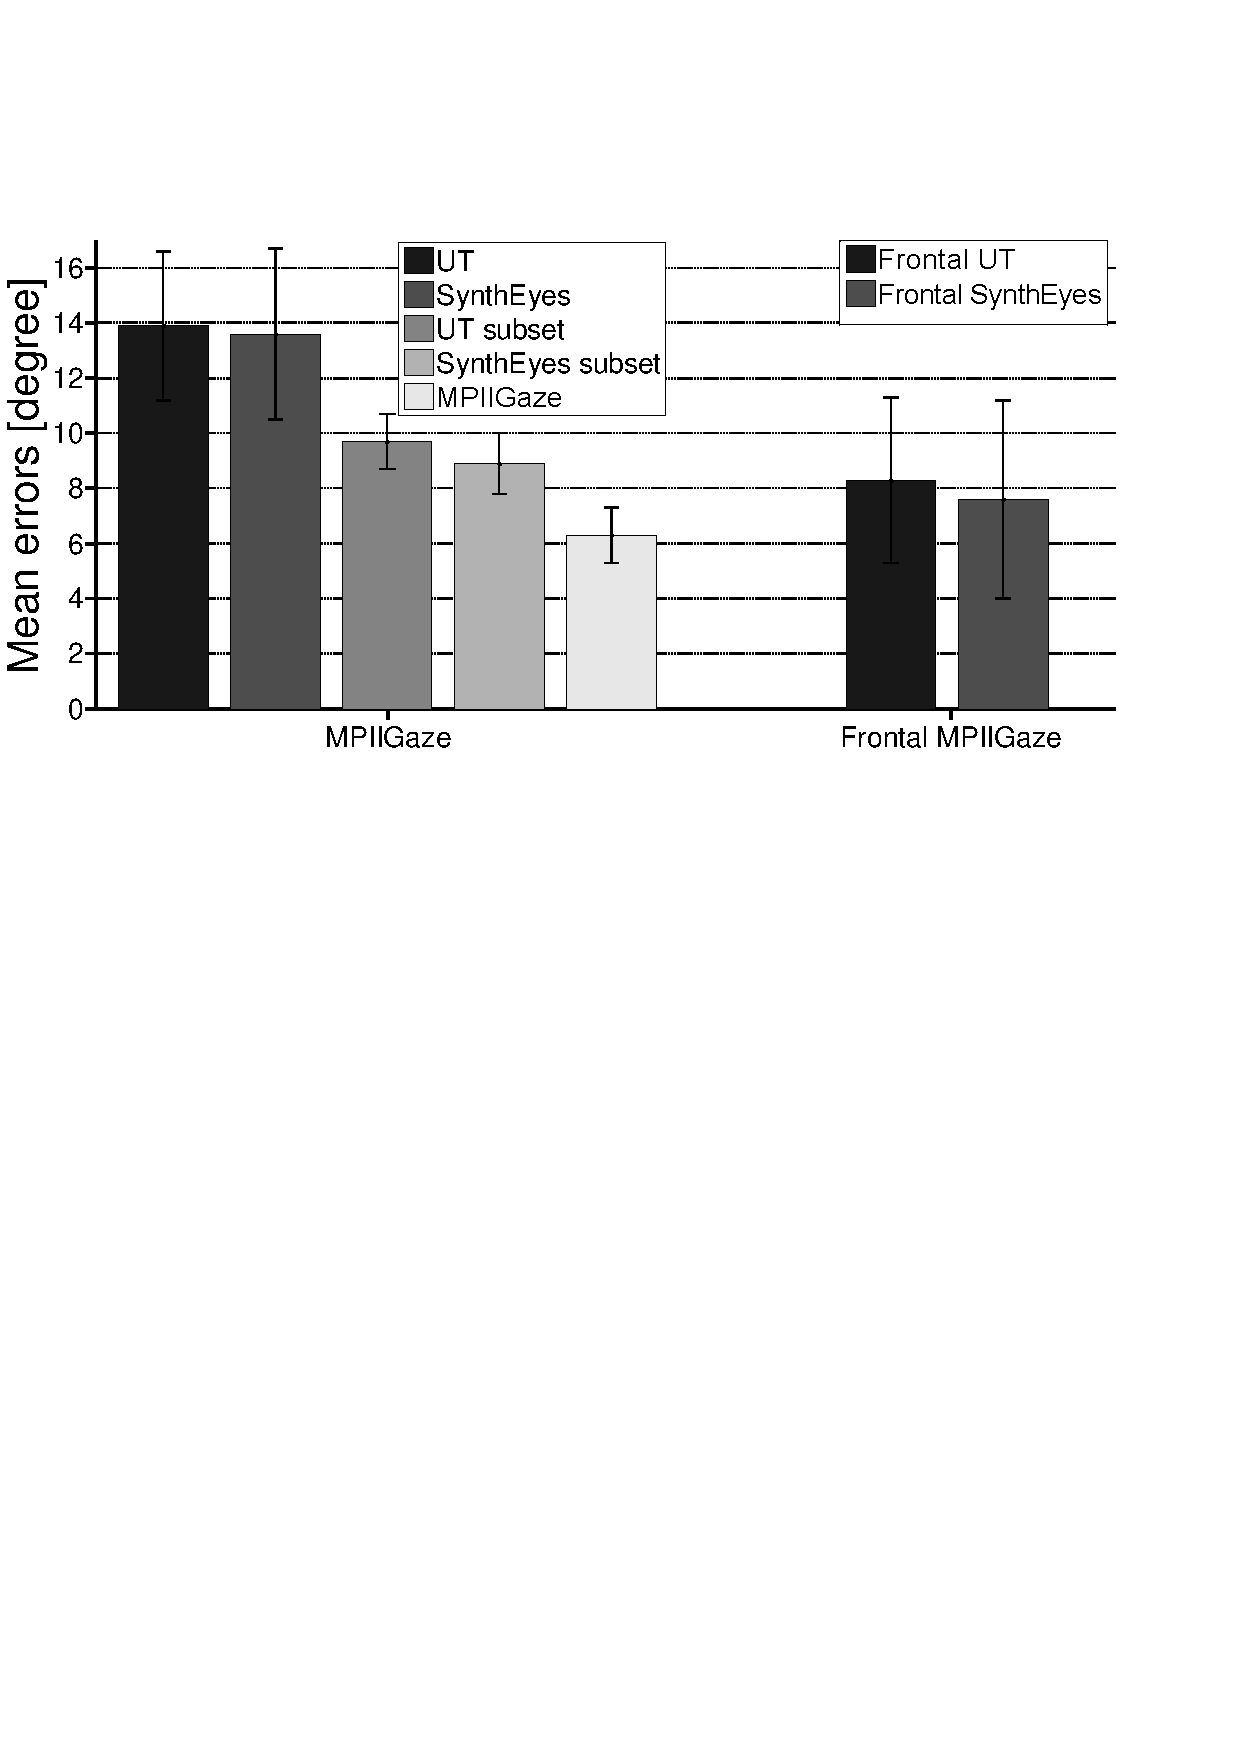
\includegraphics[width=\columnwidth]{gazeResult.pdf}
    \caption{Gaze estimation performance comparison. The X axis indicates the test set is the MPIIGaze dataset or its frontal pose subset. The legend shows different training sets.}
    \label{fig:gazeResult}
\end{figure}

To evaluate the usage of our method on appearance gaze estimation, we perform the cross-dataset validation as described in Zhang et al.~\cite{zhang15_cvpr}, where they train and test the model on different datasets. Following the same setting, we train the same Convolutional Neural Network (CNN) model on the generic~\dataset dataset, and test it on MPIIGaze evaluation subset proposed by~\cite{zhang15_cvpr}. As shown with the two bars at the far left of \autoref{fig:gazeResult}, compared to the mean gaze direction prediction error 13.9 degrees that trained with UT dataset~\cite{sugano2014learning}, the model trained with our generic~\dataset dataset can achieve the same performance with 14.0 degrees mean error. It confirms that our method can generate a equivalent data for the appearance-based gaze estimation training.

The head pose and gaze direction range are also quite important priors for appearance-based gaze estimation. Since the samples from the small range of head poses can be trained together, while extreme head poses wouldn't share eye appearance. Also the gaze direction space is arbitrary and difficult to be densely covered by collected dataset. 
We render a~\dataset subset that matches the gaze and pose distribution of MPIIGaze dataset, with added 3D laptop screen emitting light. Notice that the head pose and gaze direction range can be estimated based on the task, so the required information is not sophisticated. This shows how we can target specific scenarios like laptop-based gaze estimation, and render a suitable dataset within a day rather than taking 3 months of data collection with 15 participants. For comparison, we also re-sample a subset of UT dataset that has the same gaze and head pose distribution with MPIIGaze. Since there are just have 10 subjects in our~\dataset, we divide the UT Multiview subset into 5 groups with 10 subjects. Each group of this UT subset has 15,000 samples as with our~\dataset subset. We then average the performance of the 5 groups for the final result. 
As shown in the third and forth bars of~\autoref{fig:gazeResult}, having the similar head pose and gaze direction ranges of target domain can significantly improve the performance. And also our~\dataset subset is a better training set compared to UT subset. Since both UT subset and~\dataset subset have the same head pose and gaze direction range, the performance gains should come from the realistic samples generate from precis 3D eye model and also simulated variant appearance caused by light conditions.
The fifth bar of~\autoref{fig:gazeResult} shows the person-independent validation within the MPIIGaze dataset to show the up bounder of this scenario.


% train on synthesised images and show competitive performance on MPIIgaze with real images
% show better performance than UT dataset
%Using Xucong's CNN sytem, we train on targeted version of \dataset, test on MPII. Show results are better than training on UT and testing on MPII. This shows that the range of lighting in \dataset is important for better results.

% does photorealistic data really help/is it necessary? either reduce quality and see how it affects performance, or compare model with and without shape variations
% ^ I am not really sure how to do this well... Because we'd also have to have a measure of "how photorealistic" something is. Swapping the eyeball for a simpler model, e.g. sphere might not really have that much of an effect on "photorealism" for many eye-poses. Changing the shaders, e.g. pretending the skin is Lambertian (diffuse) might?

